% !TeX root = ../main.tex

\chapter{WeiPipe: 面向长上下文训练的通信高效权重流水线并行方法}

\section{本章概述}

随着大语言模型向长上下文方向发展，训练阶段的通信开销急剧增长，成为制约训练效率的核心瓶颈。传统的流水线并行方法采用"传递激活值"的范式，其通信量与batch size、序列长度和隐藏层维度成正比。当序列长度从4K扩展到128K时，激活值通信量增长32倍，可能使通信时间超过计算时间。在互联带宽受限的集群环境中，这一问题尤为突出。

本章提出了权重流水线并行新范式WeiPipe，突破了传统流水线并行"传递激活值"的范式，首创"传递权重"的新模式。WeiPipe将通信量从与序列长度和模型大小相关，解耦为仅与模型大小相关，从根本上解决了长序列训练的通信瓶颈问题。本章详细阐述了权重流水线并行的理论基础、WeiPipe-Naive基础策略、WeiPipe-Interleave交错式调度策略以及WeiPipe-zero-bubble零气泡调度策略，并通过实验验证了其在长序列场景下的显著性能优势。

\section{问题分析与动机}

\subsection{长上下文训练的通信挑战}

基于Transformer的大模型已成为自然语言处理、计算机视觉等多个领域的基础架构。随着研究者追求更好的性能，模型规模在两个维度上显著增长。首先，模型参数规模大幅增长。例如Llama-3.1模型拥有4050亿参数，需要至少6480 GB的GPU显存来容纳模型参数。其次，由于序列长度的增加，训练过程中的激活值规模也大幅增长。在自然语言处理领域，长上下文能力对于多轮对话、摘要生成和处理大型代码库等任务至关重要。

\begin{figure}[!t]
    \centering
    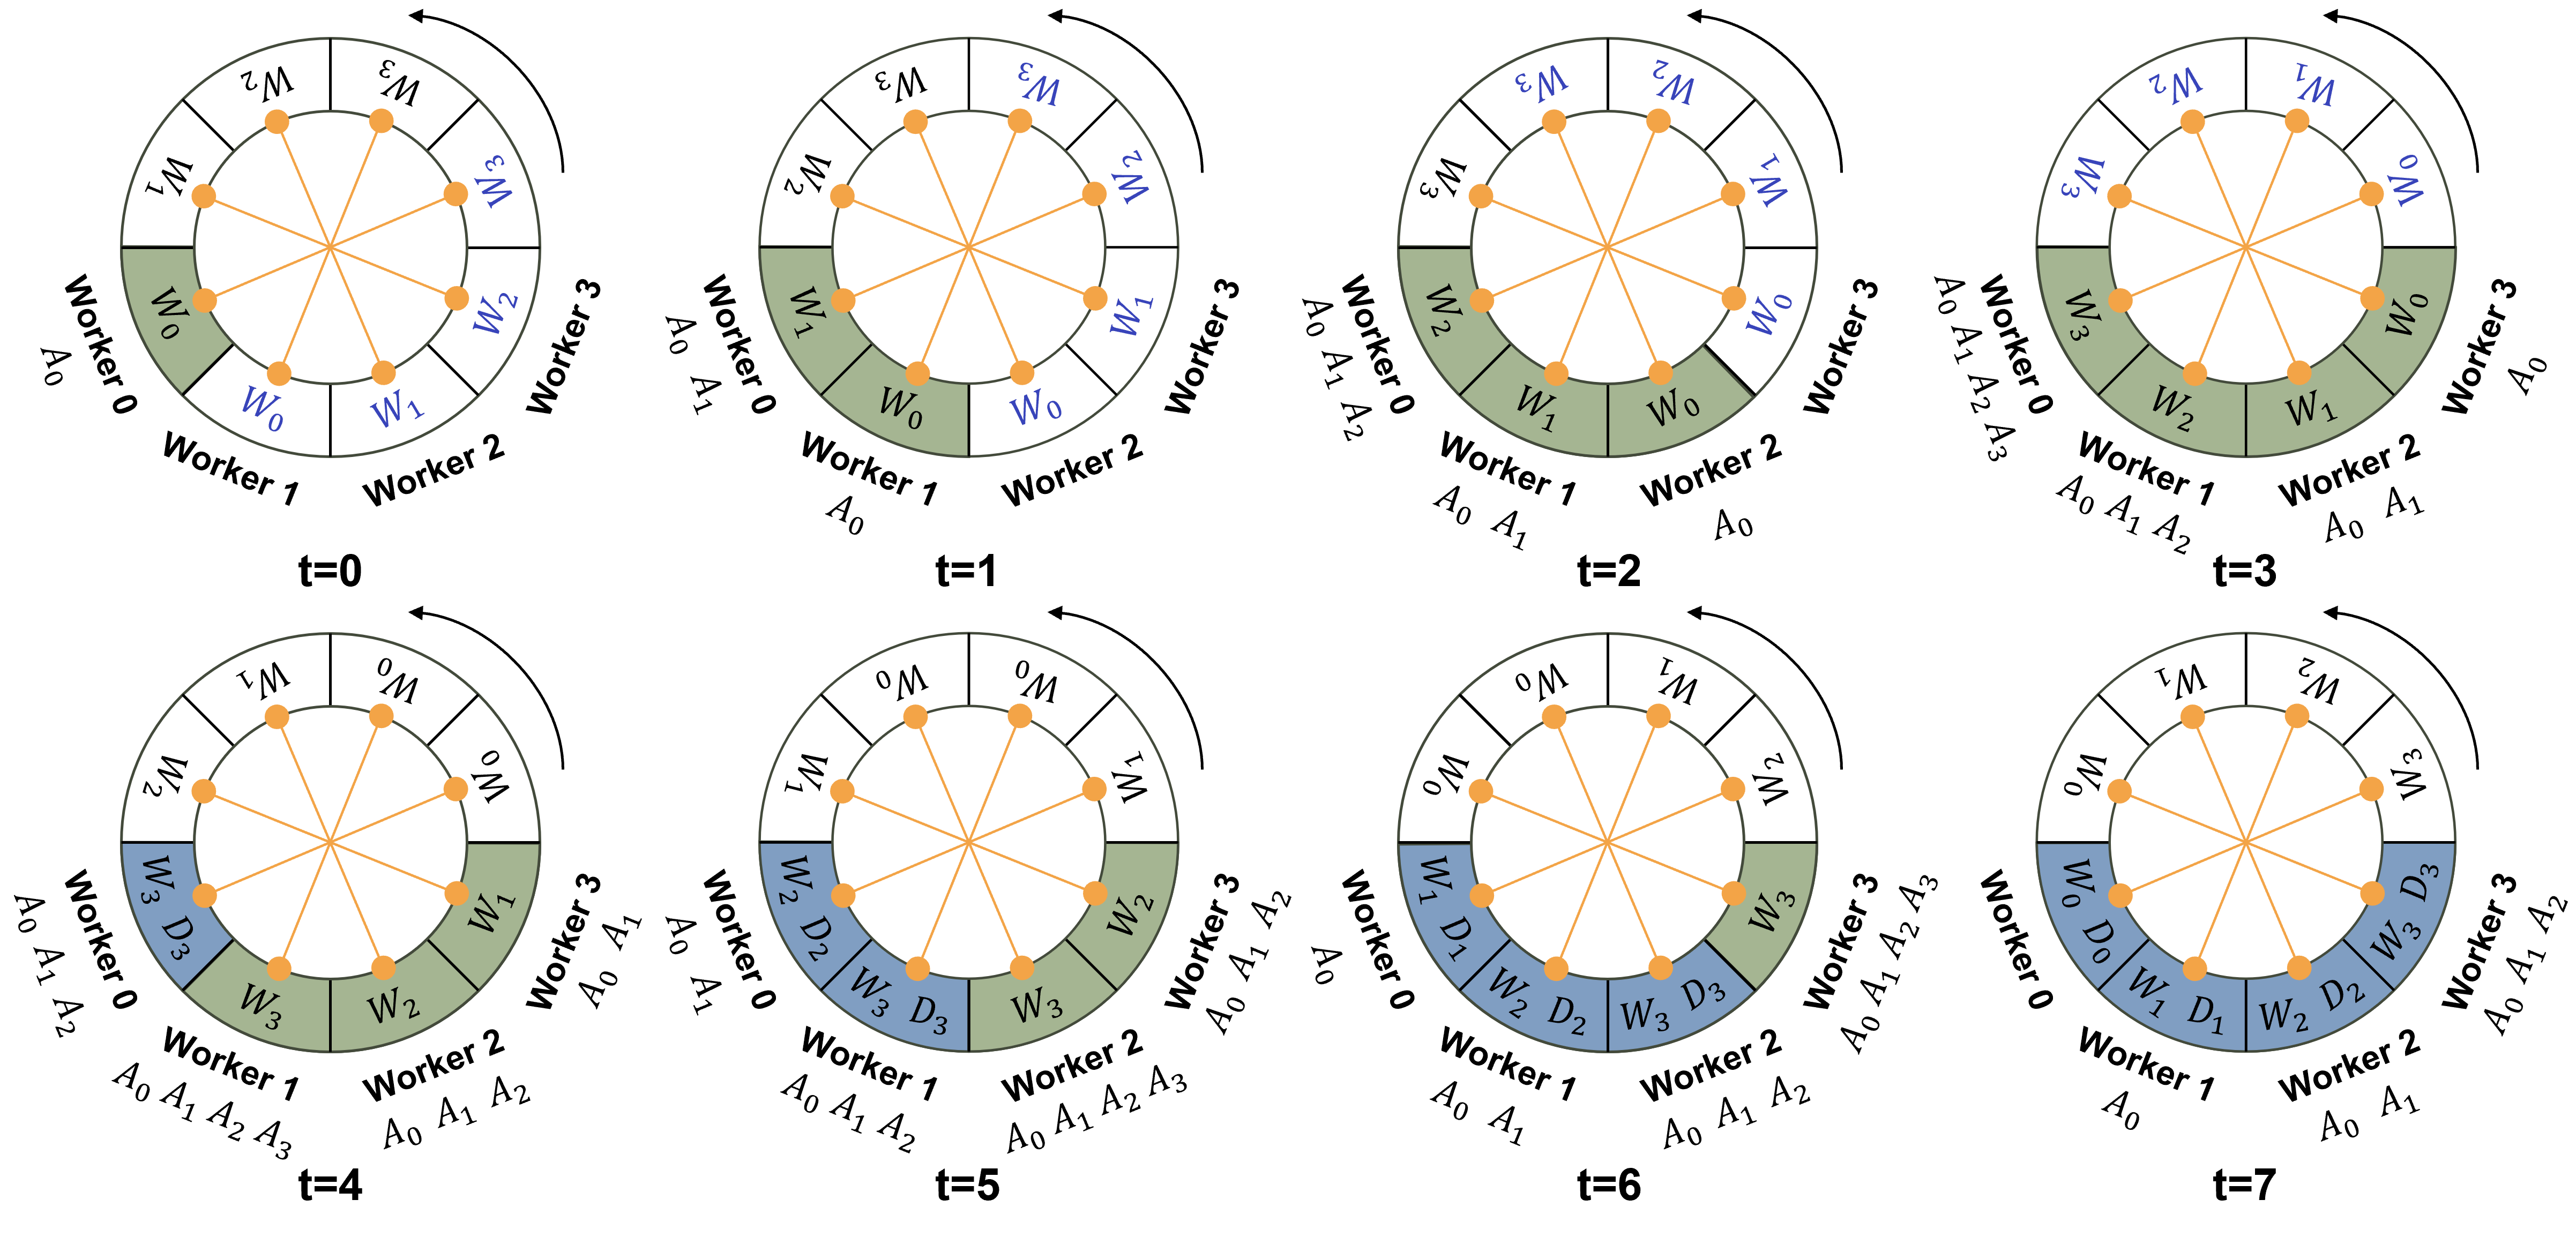
\includegraphics[width=\columnwidth]{figures/fig1.png}
    \caption{不同序列长度下激活值与权重的通信量对比。随着序列长度增长，传统流水线并行的激活值通信量急剧增加，而权重通信量保持不变。}
    \label{fig:weipipe-motivation}
\end{figure}

长上下文场景给并行策略设计带来了新挑战。传统的流水线并行（PP）将模型按层切分为多个阶段，每个设备负责一个阶段的计算，使用点对点（P2P）通信在设备间传递激活值。激活值的规模与batch size、序列长度和隐藏层维度成正比。

如图\ref{fig:weipipe-motivation}所示，随着序列长度的增加，传统流水线并行需要传递的激活值规模急剧增长。当序列长度从4K扩展到128K时，激活值通信量增长32倍，可能使通信时间超过计算时间。

以LLaMA风格的模型为例，单个Transformer阶段的输出激活值大小约为$GSH$（以元素数计），其中$G$是micro-batch size，$S$是序列长度，$H$是隐藏层维度。相比之下，单层模型的权重大小约为$12H^2$，包括注意力模块的$4H^2$和前馈网络（FFN）的$8H^2$。当输出激活值与权重的比值$\frac{GS}{12H}$超过1时，传递权重的方法在通信上比传递激活值更高效。

以具体数值为例：当$H=4096$，$S=16384$，$G=32$时，$\frac{GS}{12H}=\frac{32 \times 16384}{12 \times 4096} \approx 10.67$，意味着传递激活值的通信量是传递权重的10倍以上。这为设计新的流水线范式提供了强有力的动机。

\subsection{内存优化技术对通信的影响}

混合精度训练、梯度检查点（gradient checkpointing）和FlashAttention等内存优化技术已成为大模型训练的标准配置。这些技术降低了峰值内存占用，允许使用更大的batch size，但同时也增加了需要传递的数据量。

具体而言：
\begin{itemize}
    \item \textbf{混合精度训练}：使用FP16/BF16存储激活值，降低存储开销，但不改变通信量的相对比例。
    \item \textbf{梯度检查点}：通过在反向传播时重新计算部分激活值来节省内存。这减少了前向传播时需要存储的激活值，但增加了计算量，且不影响设备间传递的激活值规模。
    \item \textbf{FlashAttention}：优化注意力计算，大幅降低注意力模块的内存占用。这允许更大的batch size和更长的序列长度，但同时也增加了流水线并行中需要传递的激活值规模。
\end{itemize}

这些技术的采用使得传统流水线并行面临更严峻的通信压力，进一步凸显了重新设计通信模式的必要性。

\subsection{现有方法的局限性}

现有的并行策略在长序列场景下各有局限：

\textbf{数据并行（DP）及其变体}：ZeRO系列（ZeRO-1/2/3，即FSDP）通过分片优化器状态、梯度和参数来降低显存占用。然而，ZeRO系列显著增加了通信量，每次前向和反向传播都需要多次all-gather和reduce-scatter操作。在互联带宽受限的环境中，通信开销可能成为瓶颈。

\textbf{张量并行（TP）}：将单个算子切分到多个设备并行执行。TP需要频繁的all-reduce同步，对互联带宽要求极高，通常仅在NVLink互联的节点内部使用。

\textbf{传统流水线并行（PP）}：包括GPipe、1F1B、Chimera、Zero-Bubble等策略。这些方法主要关注优化流水线气泡率，但都采用"传递激活值"的范式，在长序列场景下面临通信瓶颈。

综上所述，现有技术无法有效解决长上下文场景下的通信瓶颈问题，特别是对于互联带宽受限的集群环境。这促使我们探索新的流水线范式——传递权重而非激活值。

\section{权重流水并行机制}

\subsection{核心思想和理论推导}

WeiPipe的核心思想是：在流水线并行中，让模型权重而非激活值在设备间流转。这一范式转换带来以下优势：

\textbf{通信量解耦}：传统PP的通信量为$O(GSH)$，与batch size和序列长度成正比。WeiPipe的通信量为$O(H^2)$，仅与模型隐藏层维度相关，与batch size和序列长度无关。

\textbf{通信模式简单}：WeiPipe仅依赖点对点（P2P）通信，不需要集体通信原语（如all-reduce、all-gather），便于在带宽受限的环境中扩展。

\textbf{内存均衡}：WeiPipe中每个worker存储所有层的激活值（针对单个micro-batch），而非传统PP中存储单个阶段的多个micro-batch激活值。这使得内存使用在设备和时间上更加均衡。

以环形拓扑为例，假设层数$L$等于worker数$P$，每个worker持有单层的权重。训练过程包含三个阶段：前向传播、反向传播和更新阶段。

\subsection{WeiPipe-Naive：基础权重流转策略}

WeiPipe-Naive是权重流水线并行的基础形式，用于演示核心机制。

\begin{figure}[!t]
    \centering
    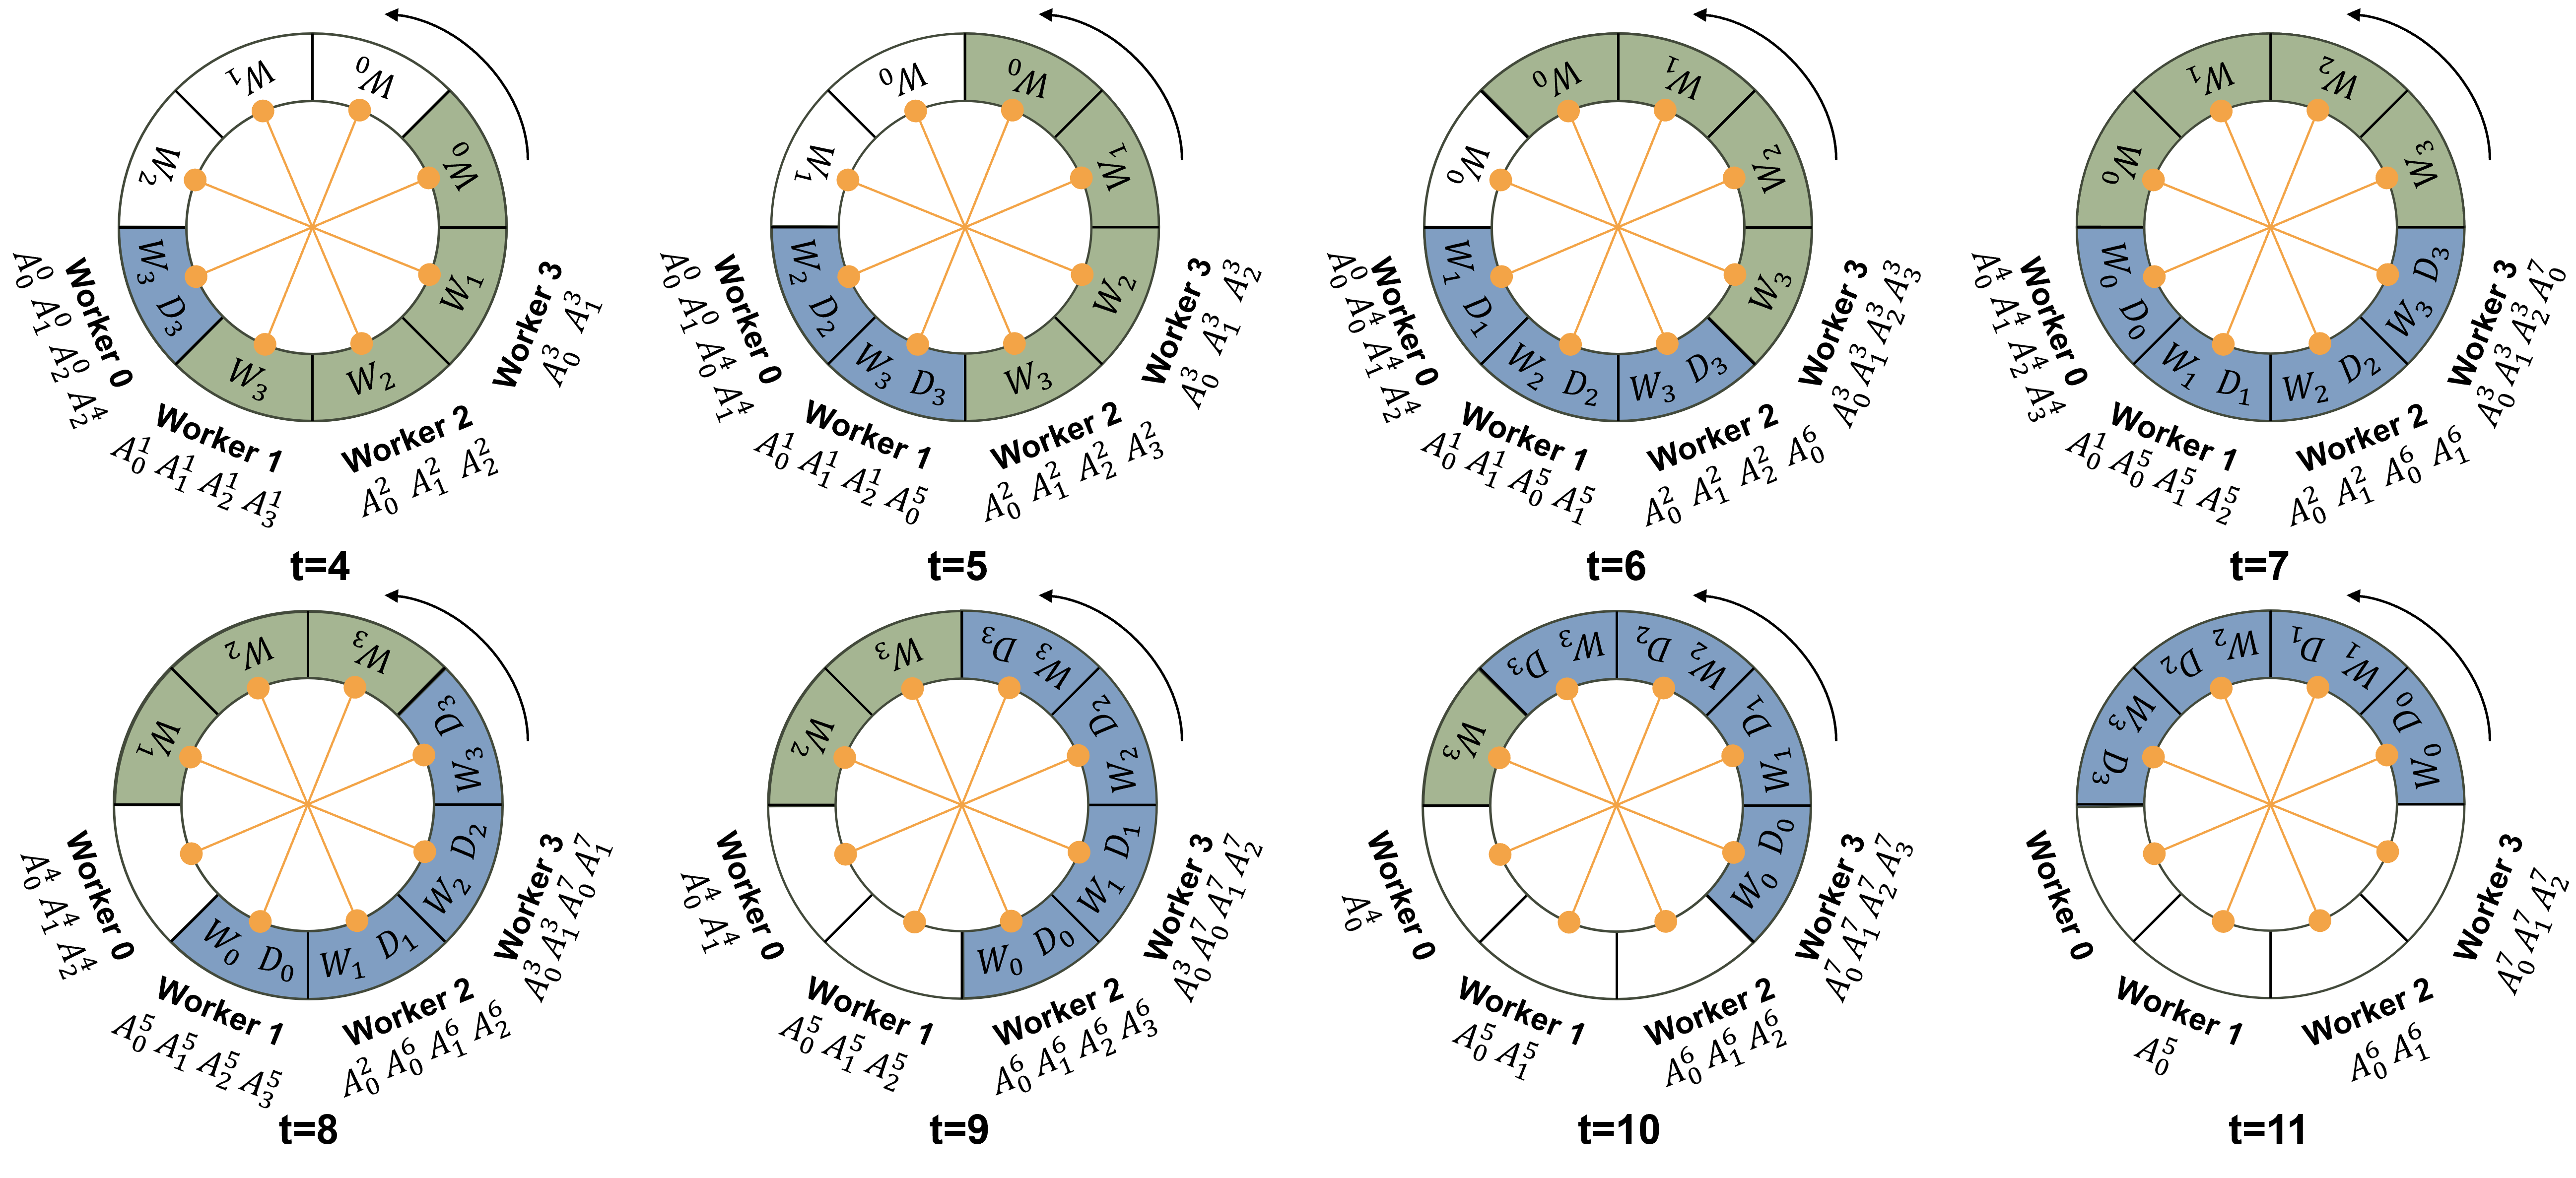
\includegraphics[width=\columnwidth]{figures/fig2.png}
    \caption{WeiPipe-Naive基础权重流转策略示意图。权重在环形拓扑的worker间流转，每个worker持有单层权重并依次处理所有层。}
    \label{fig:weipipe-naive}
\end{figure}

如图\ref{fig:weipipe-naive}所示，WeiPipe-Naive在环形拓扑中实现权重流转。假设层数$L$等于worker数$P$，每个worker持有单层的权重。

\textbf{前向传播阶段}：Worker 0持有第一层的权重$W_0$，启动前向计算。同时，它将$W_0$传递给Worker 1，并从Worker $P-1$接收$W_1$。随后，Worker 0丢弃$W_0$但保留第一层的激活值$A_0$，开始使用$W_1$进行第二层的前向计算。与此同时，Worker 1使用新的micro-batch输入计算第一层。这一过程持续直到Worker 0完成所有层的前向传播。

\textbf{反向传播阶段}：反向传播更为复杂，因为权重需要以逆序使用。为了保持权重流水，我们在环的另一侧填充$W_3$到$W_0$。当Worker 0完成前向传播后，环继续逆时针旋转。Worker 0依次接收$W_3$到$W_0$并执行从第3层到第0层的反向计算。在WeiPipe-Naive中，索引较小的worker较早完成，因此可能需要同时传递前向和反向的权重。

\textbf{更新阶段}：每个worker使用权重梯度（$D$s）更新权重。由于权重在worker间循环，每个worker只生成其micro-batch的$D$片段。更新一层权重需要收集所有对应的$D$s。与DP中使用all-reduce原语不同，WeiPipe旨在仅使用P2P通信，因此$D$s也通过环循环传递。每个处理该层反向传播的worker将新生成的$D$与现有的$D$进行平均、求和或归一化，并保持通信量不变。这一循环过程重复直到所有micro-batch处理完成。

WeiPipe-Naive存在明显的缺陷：同时有两个权重流循环，但只有一个用于当前计算，导致冗余权重传输增加通信开销。更重要的是，反向传播的计算时间约为前向传播的两倍，当一个worker执行反向传播时，会显著增加其他正在执行前向传播的worker的流水线气泡。这些缺陷促使我们设计更高级的调度策略。

\section{高级调度策略设计}

\subsection{WeiPipe-Interleave：交错式权重流水策略}

为了解决WeiPipe-Naive的问题，我们提出WeiPipe-Interleave策略，通过交错前向和反向传播来降低气泡率和通信需求。

\begin{figure}[!t]
    \centering
    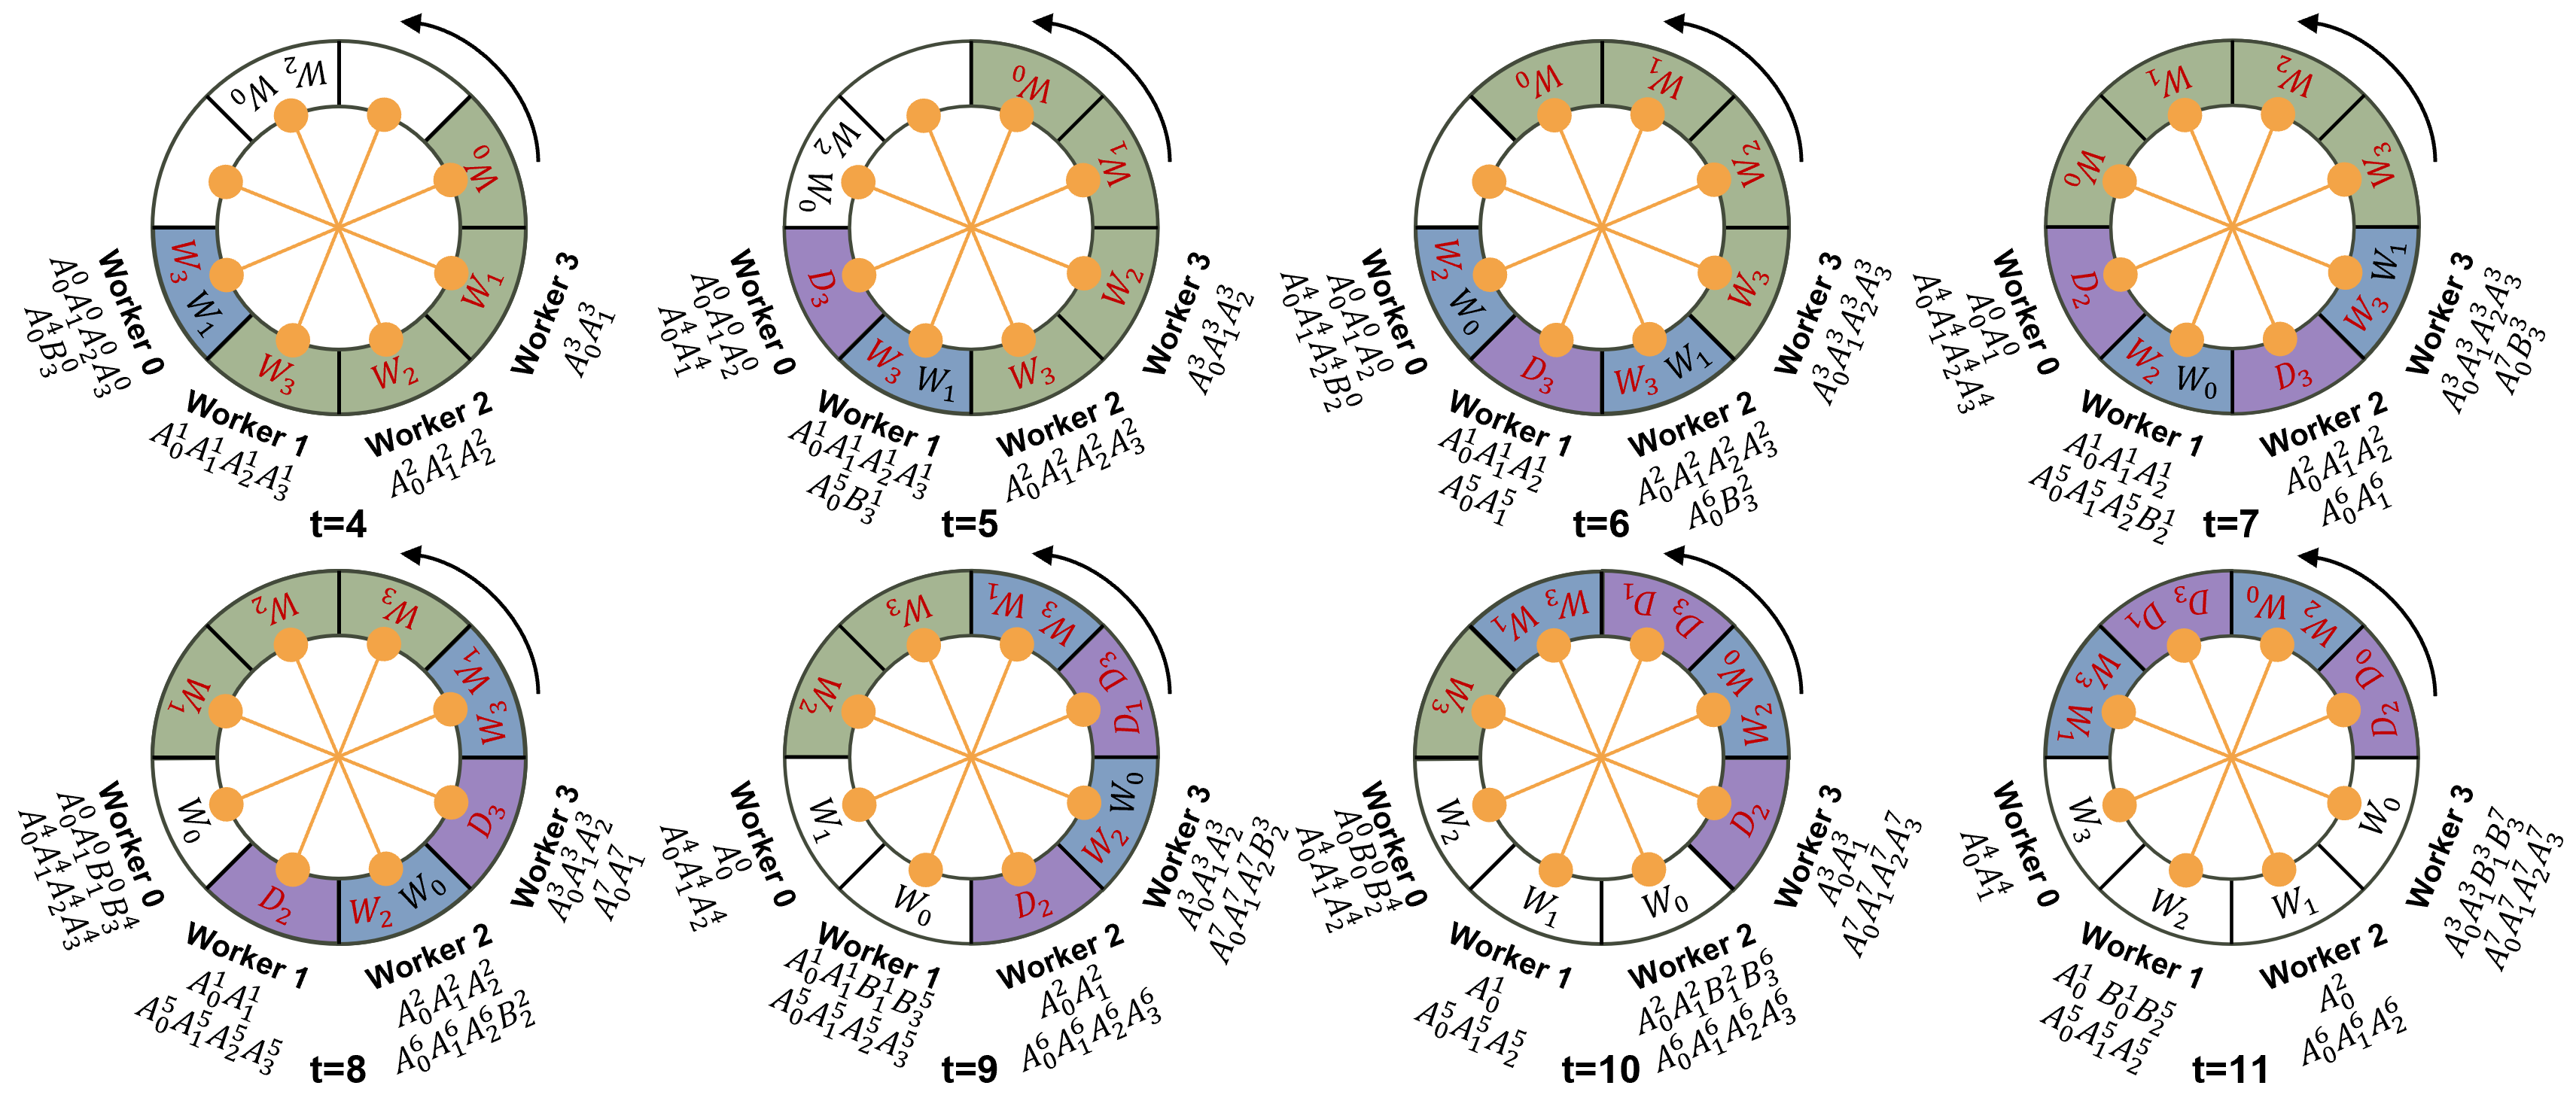
\includegraphics[width=\columnwidth]{figures/fig3.png}
    \caption{WeiPipe-Interleave交错式权重流水策略示意图。通过在前向-反向交错阶段同时执行两种计算，消除了流水线气泡。}
    \label{fig:weipipe-interleave}
\end{figure}

如图\ref{fig:weipipe-interleave}所示，核心思想是利用环对角位置的权重进行另一个micro-batch的前向或反向计算。初始前向过程与WeiPipe-Naive相同。当Worker 0开始反向传播时，同时利用$W_0$执行新micro-batch输入的前向传播。因此，在此位置，Worker 0将在环转动一次之前执行一次反向和一次前向计算。与此同时，其他worker只能执行一次前向操作并等待Worker 0的计算完成。在随后的转动中，当计算负载在worker间平衡时，Worker 0到3也进入前向-反向交错阶段。

在前向-反向交错阶段，无论前向和反向的工作负载差异如何，都没有流水线气泡。每个worker还可以根据其数据传输情况自行决定前向和反向传播的执行顺序。此外，前向和反向传播期间的空闲内存被用于存储新micro-batch生成的激活值，实现了不同worker和时间点上的均衡存储利用。

WeiPipe-Interleave进一步降低了通信开销。对于LLaMA结构（单层参数量为$12H^2$），在前向-反向交错阶段，每个worker每轮接收两层权重和一层$D$。通信量为$36H^2$，相比WeiPipe-Naive计算/通信比翻倍。

\subsection{WeiPipe-zero-bubble：零气泡权重流水策略}

为了进一步探索权重流水线的潜力，我们提出了WeiPipe与零气泡流水线的结合方案。零气泡策略将反向计算拆分为B-pass（计算激活梯度）和W-pass（计算权重梯度），可以实现接近零气泡的理想状态。

\begin{figure}[!t]
    \centering
    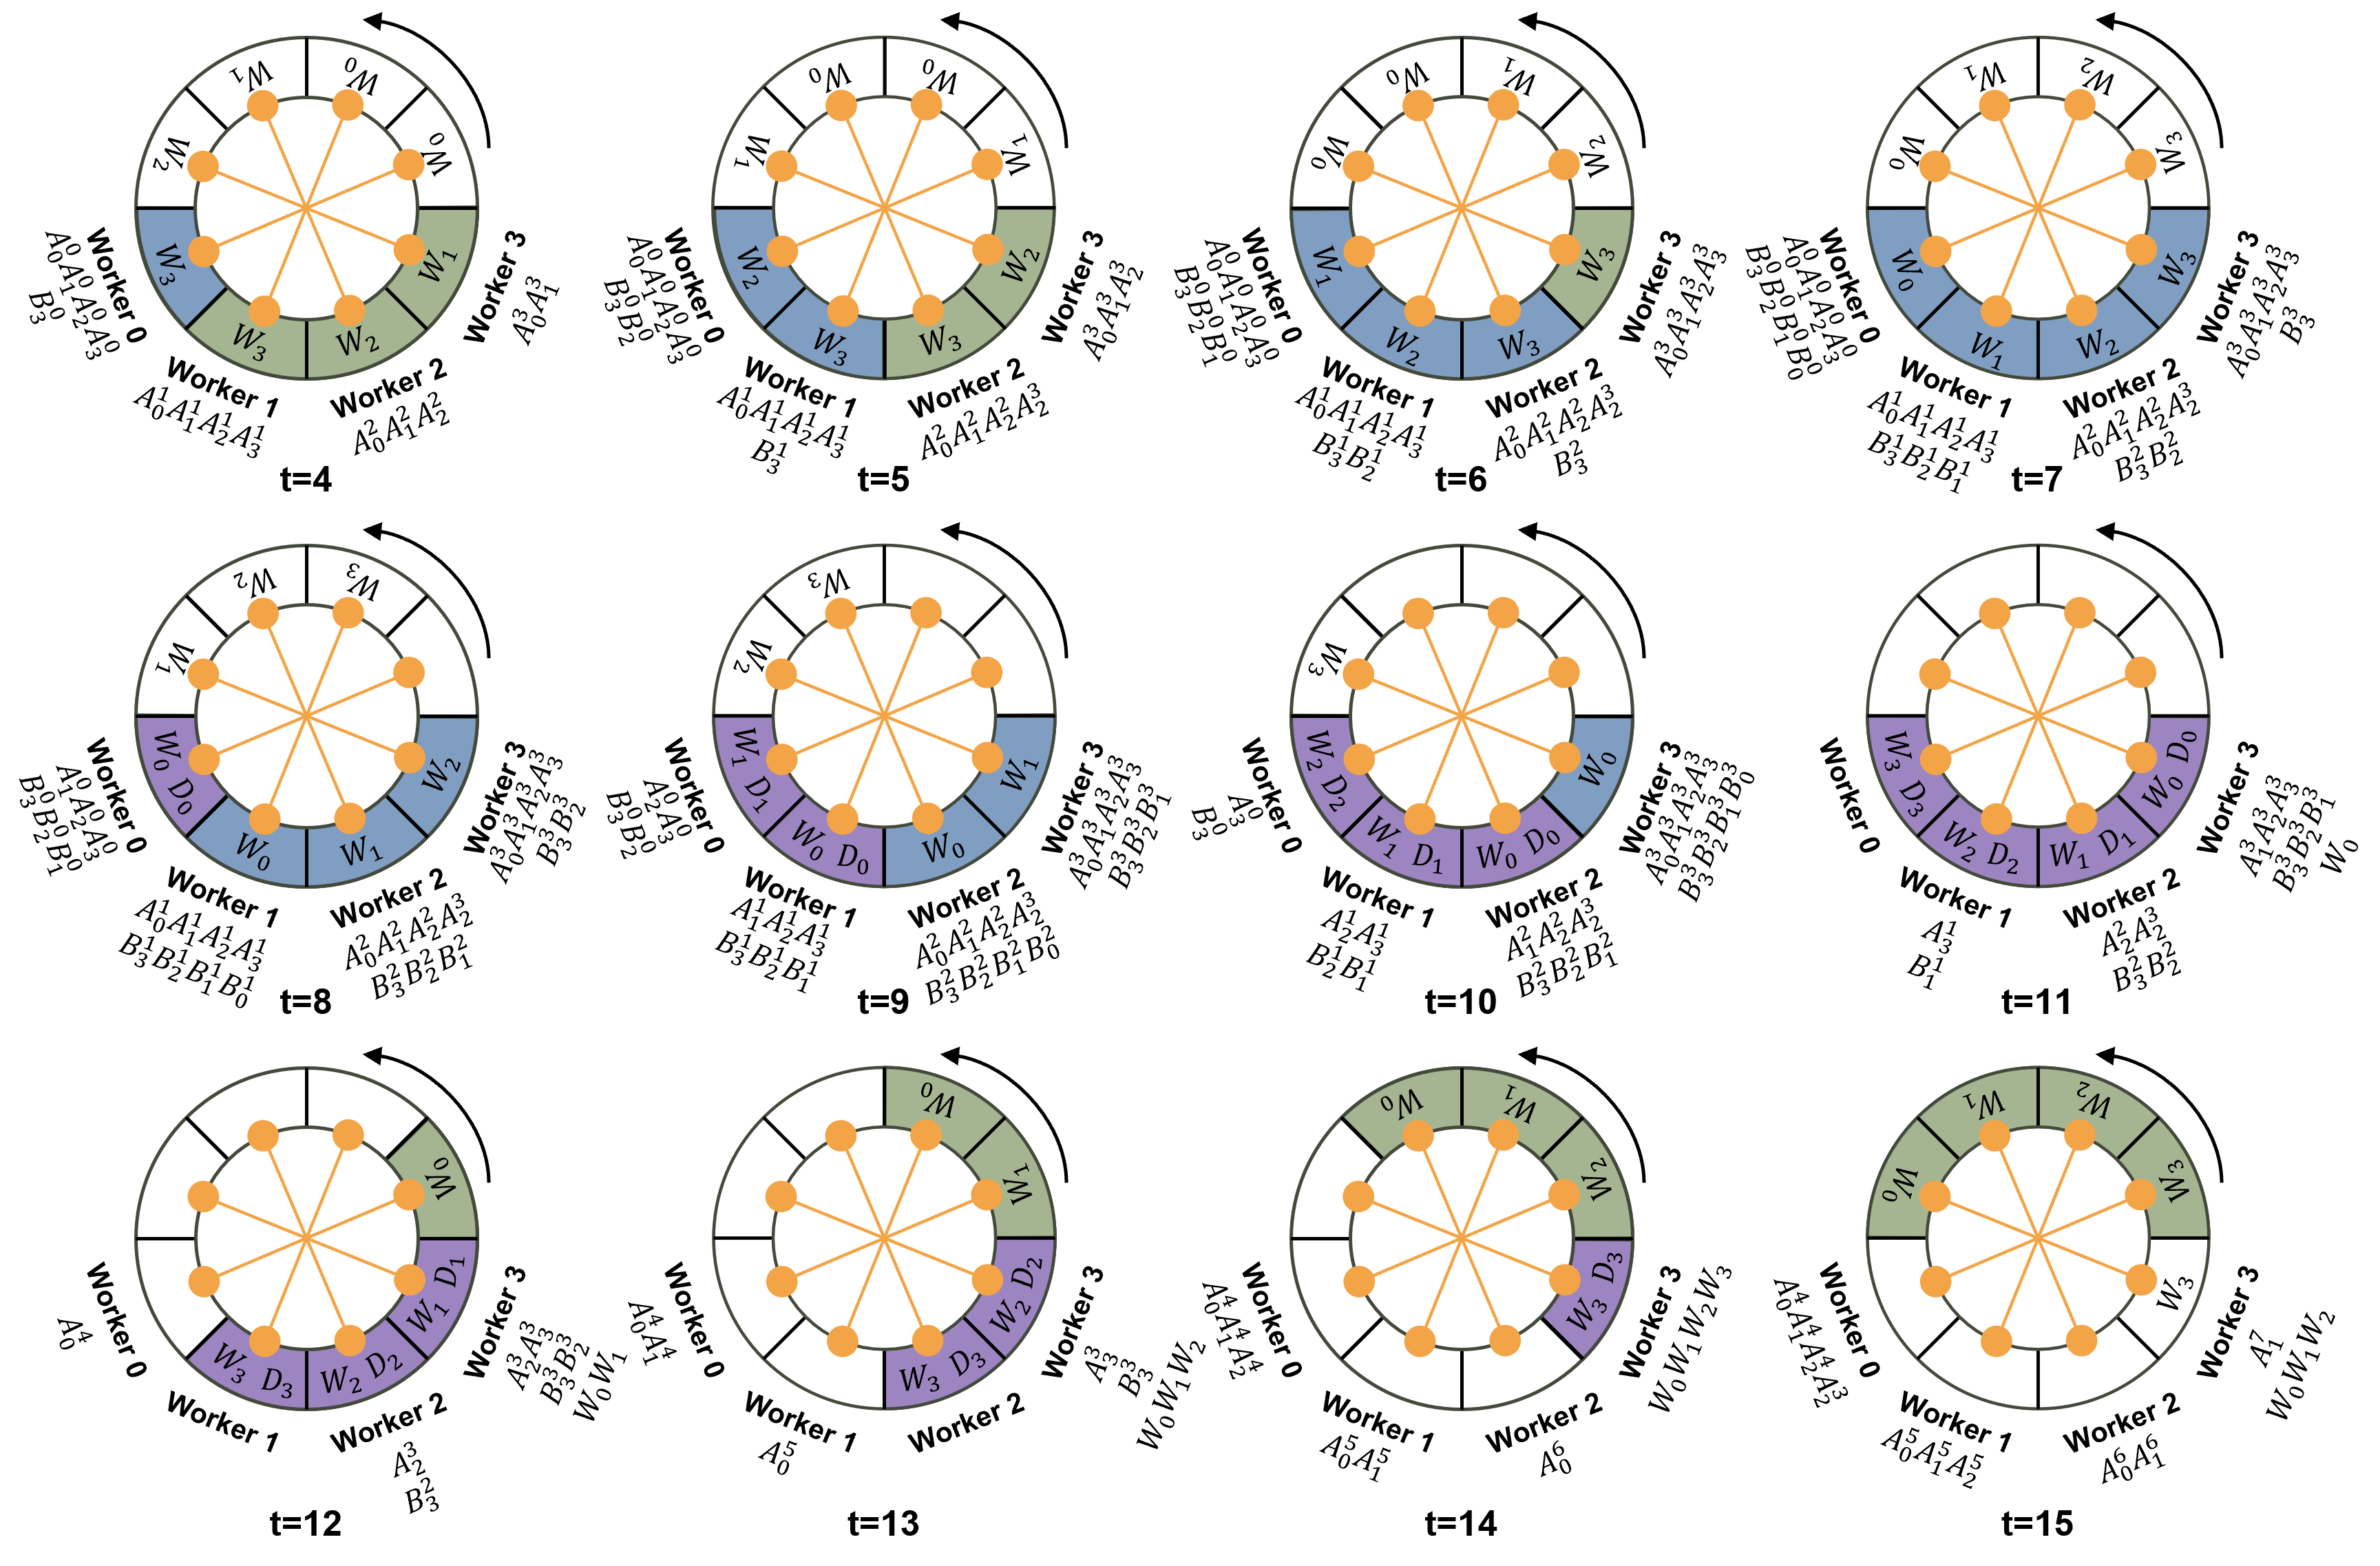
\includegraphics[width=\columnwidth]{figures/fig4.png}
    \caption{WeiPipe-zero-bubble策略示意图。通过将反向传播拆分为B-pass和W-pass，结合权重流转实现接近零气泡的调度。}
    \label{fig:weipipe-zerobubble}
\end{figure}

如图\ref{fig:weipipe-zerobubble}所示，我们引入两种变体：

\textbf{WeiPipe-zero-bubble 1 (WZB1)}：在WeiPipe-Interleave基础上略微降低气泡率，存储和通信开销相对较低。在前向传播阶段，权重安排与之前策略一致。B-pass和W-pass的权重以及W-pass生成的梯度成对放置。对于$L$层的网络，$W_{L-1}$与$W_{L/2-1}$放在一起，$W_{L-2}$与$W_{L/2-2}$放在一起，以此类推。这种安排确保每个worker在一轮内执行2块操作，同时向下一个worker传输3块数据。峰值内存约为$1.5GM_A$。

\textbf{WeiPipe-zero-bubble 2 (WZB2)}：实现接近零气泡的配置。所有层的前向、B-pass和W-pass在一个worker内顺序执行。特别地，W-pass从第0层到第3层进行，与前向顺序匹配。最后一个worker（Worker 3）聚合所有$D$s并更新权重。这种无缝交接允许使用更少的micro-batch进行频繁权重更新，实现几乎零气泡。WZB2的通信和存储开销较高，每执行1块操作需要向下一个worker传输2块数据。

\section{理论分析}

\subsection{气泡率比较}

流水线并行的气泡率定义为气泡时间占总迭代时间的比例。对于经典1F1B，气泡率为$(P-1)/(N+P-1)$，其中$P$为流水线阶段数，$N$为micro-batch数量。

WeiPipe-Interleave的气泡率与1F1B相同。这是因为两者都采用类似的前向-反向交错调度，WeiPipe-Interleave通过让worker在反向传播阶段同时处理新的前向micro-batch，保持了与1F1B一致的设备利用率。

对于两种零气泡策略，其气泡率通过在气泡率公式中将$N$替换为$N \cdot k$（$k>1$）来降低，即通过增加有效micro-batch数量来稀释固定的启动和排空开销。ZB2和WZB2进一步细化了B-pass和W-pass的调度，在理想情况下（$N$足够大）可以实现接近零气泡的理想状态。然而，零气泡策略的代价是显著增加的内存占用，这在实际长上下文场景中可能引发OOM错误。

\subsection{通信效率分析}

通信效率通过接收的总数据量除以计算时间（带宽使用率）来评估。不同流水线策略的不同区域有不同的通信密度。

对于传递激活值的PP，中间worker需要传递激活值$A$和对应梯度$B$，因此公式中有系数"2"。以LLaMA风格模型为例，单个Transformer阶段的输出激活值大小约为$GSH$（元素数），因此传递激活值的单向通信量约为$2GSH$。传递激活值策略的通信量随micro-batch size $G$和序列长度$S$线性增长，在长序列场景下这一增长是决定性的。

相比之下，WeiPipe的通信量仅由权重数量决定，与$G$和$S$无关。对于LLaMA结构，单层参数量为$12H^2$（注意力模块$4H^2$+FFN模块$8H^2$）。WeiPipe-Interleave需要传输两块$W$和一块$D$（梯度），每轮通信量为$36H^2$，持续时间为$\frac{T_F + T_B}{P}$，其中$T_F$和$T_B$分别为完整前向和反向传播时间。

对比两种策略的通信量：
\begin{itemize}
    \item 传递激活值PP（中间worker）：通信量 $\approx \frac{2GSH}{\frac{T_F+T_B}{P}} = \frac{2GSHP}{T_F+T_B}$
    \item WeiPipe-Interleave：通信量 $= \frac{36H^2}{\frac{T_F+T_B}{P}} = \frac{36H^2 P}{T_F+T_B}$
\end{itemize}

因此，当$\frac{GS}{18H} > 1$（即$GS > 18H$）时，WeiPipe-Interleave的通信效率优于传递激活值的方法。以$H=4096$，$S=16384$，$G=32$为例：$\frac{GS}{18H} = \frac{32 \times 16384}{18 \times 4096} \approx 7.1 \gg 1$，WeiPipe-Interleave的通信效率约为传统PP的7.1倍。类似地，当$\frac{GS}{27H} > 1$时，WZB1相比零气泡策略也具有通信优势。

\subsection{内存消耗分析}

内存消耗受具体实现的显著影响。这里基于$M_A$（单层激活值内存）、$M_B$（单层反向梯度内存）、$M_W$（单层权重内存）和$M_D$（单层权重梯度内存）的数量提供粗略估计，忽略通信缓冲区、嵌入层和混合精度训练等因素。

对于1F1B和WeiPipe-Interleave，主要部分是激活值存储，计为$GM_A$（$G$个micro-batch各自存储一层的激活值）。WeiPipe-Interleave的内存消耗与1F1B相似但更加均衡——在WeiPipe中，每个worker需要存储所有层的激活值（针对单个micro-batch），而非传统PP中存储单个阶段的多个micro-batch激活值。这使得内存使用在设备间和时间维度上更加均衡，避免了流水线启动时早期worker内存压力过大的问题。

在分离B-pass和W-pass的策略中，一阶段B-pass会消耗前向传播存储的部分激活值$M_A/P$，并生成梯度$M_B/P$。假设B-pass完成后剩余$\alpha M_A/P$的激活值存储，其中$\alpha$取决于具体实现和FlashAttention的使用情况。对于零气泡流水线，峰值存储需求出现在最后一个worker处：ZB1和WZB2都需要存储$G(\alpha M_A+M_B)$的数据，ZB2几乎将此需求翻倍。然而，WZB1可以实现约$1.5GM_A$的最大内存消耗，当$\frac{M_B}{M_A} > 1.5-\alpha$时，低于其他零气泡策略。

值得特别关注的是FlashAttention对零气泡策略内存需求的影响。在未使用FlashAttention时，前向传播期间的激活值主要由注意力计算产生，这部分内存在B-pass期间被释放，而生成的梯度相比之下较小，因此峰值内存通常出现在第一个worker第一次反向传播开始之前。然而，启用FlashAttention后，注意力模块的激活值大幅减少，前向传播的激活值主要来自FFN计算。此时B-pass产生的梯度大小与一次前向传播产生的激活值大小相当，导致峰值内存出现在最后一个worker执行第一次W-pass之前，约为峰值的两倍。这解释了为何在实际长上下文训练中，零气泡策略的内存消耗显著高于理论预期，容易在$S \ge 8192$的配置下出现OOM错误。

以$H=4096$，$S=4096$，$N=12$，$G=32$，$\alpha=0.6$为基准（不含重计算和FlashAttention）：WeiPipe-Interleave的内存占用与1F1B相当，而ZB1和WZB2的峰值内存约为1F1B的1.7倍，ZB2约为3.4倍。

\section{实现细节}

我们在PyTorch上从头实现了WeiPipe-Interleave。实现针对LLM训练定制，但方法不限于Transformer。以下是实现中考虑的细节：

\textbf{混合精度}：与其他主要关注全精度实现的流水线研究不同，我们的实现采用广泛使用的混合精度训练以进一步降低存储和通信。具体地，$A$、$W$和$D$使用fp16精度，$B$使用bf16。优化器状态使用fp32，分布在worker间。

\textbf{通信重叠}：WeiPipe精心调整计算和权重传递的安排，以平衡通信和计算工作负载。为确保高性能潜力，实现了通信隐藏优化。在前向-反向交错期间，使用PyTorch分布式库的batch\_isend\_irecv函数进行异步通信预取$W$s和$D$s。

\textbf{重计算和Flash Attention}：重计算（梯度检查点/重物化）是一种通过在前向传播期间放弃部分激活值来节省存储的策略。这些值在反向传播期间重新计算，以冗余计算显著降低内存消耗。类似地，Flash Attention是优化注意力模块内存访问和节省内存的广泛使用技术。通过采用这些技术，可以增加micro-batch size并增强WeiPipe的优势。

\section{实验评估}

\subsection{实验设置}

\textbf{模型配置}：基于LLaMA-2结构（也适用于GPT风格模型）进行评估。固定头数为32，层数$L$为32。改变隐藏层维度$H$、token长度$S$、micro-batch size $G$和迭代中micro-batch数量$N$以获得不同规模的模型。

\textbf{对比方法}：将WeiPipe-Interleave与广泛使用的1F1B、最先进的零气泡1和2、以及FSDP进行比较。1F1B和零气泡策略通过Megatron-LM实现，FSDP通过DeepSpeed的ZeRO-3优化实现。所有策略采用相同的模型配置、micro-batch size、混合精度设置、重计算、Flash Attention和硬件环境。

\textbf{硬件环境}：使用Colossal Cloud的A800 GPU。A800拥有80GB HBM和312 TFlops的fp16/bf16张量核心。与A100相比，A800将NVLink带宽从600GB/s限制到400GB/s。采用两种通信基础设施：（1）16个A800 GPU在两个集群内通过NVLink连接；（2）32个A800 GPU跨4个集群，集群内通过PCIe连接。集群间通过10Gb以太网连接。使用NCCL作为底层通信库。

\subsection{吞吐量和内存消耗}

\begin{figure}[!t]
    \centering
    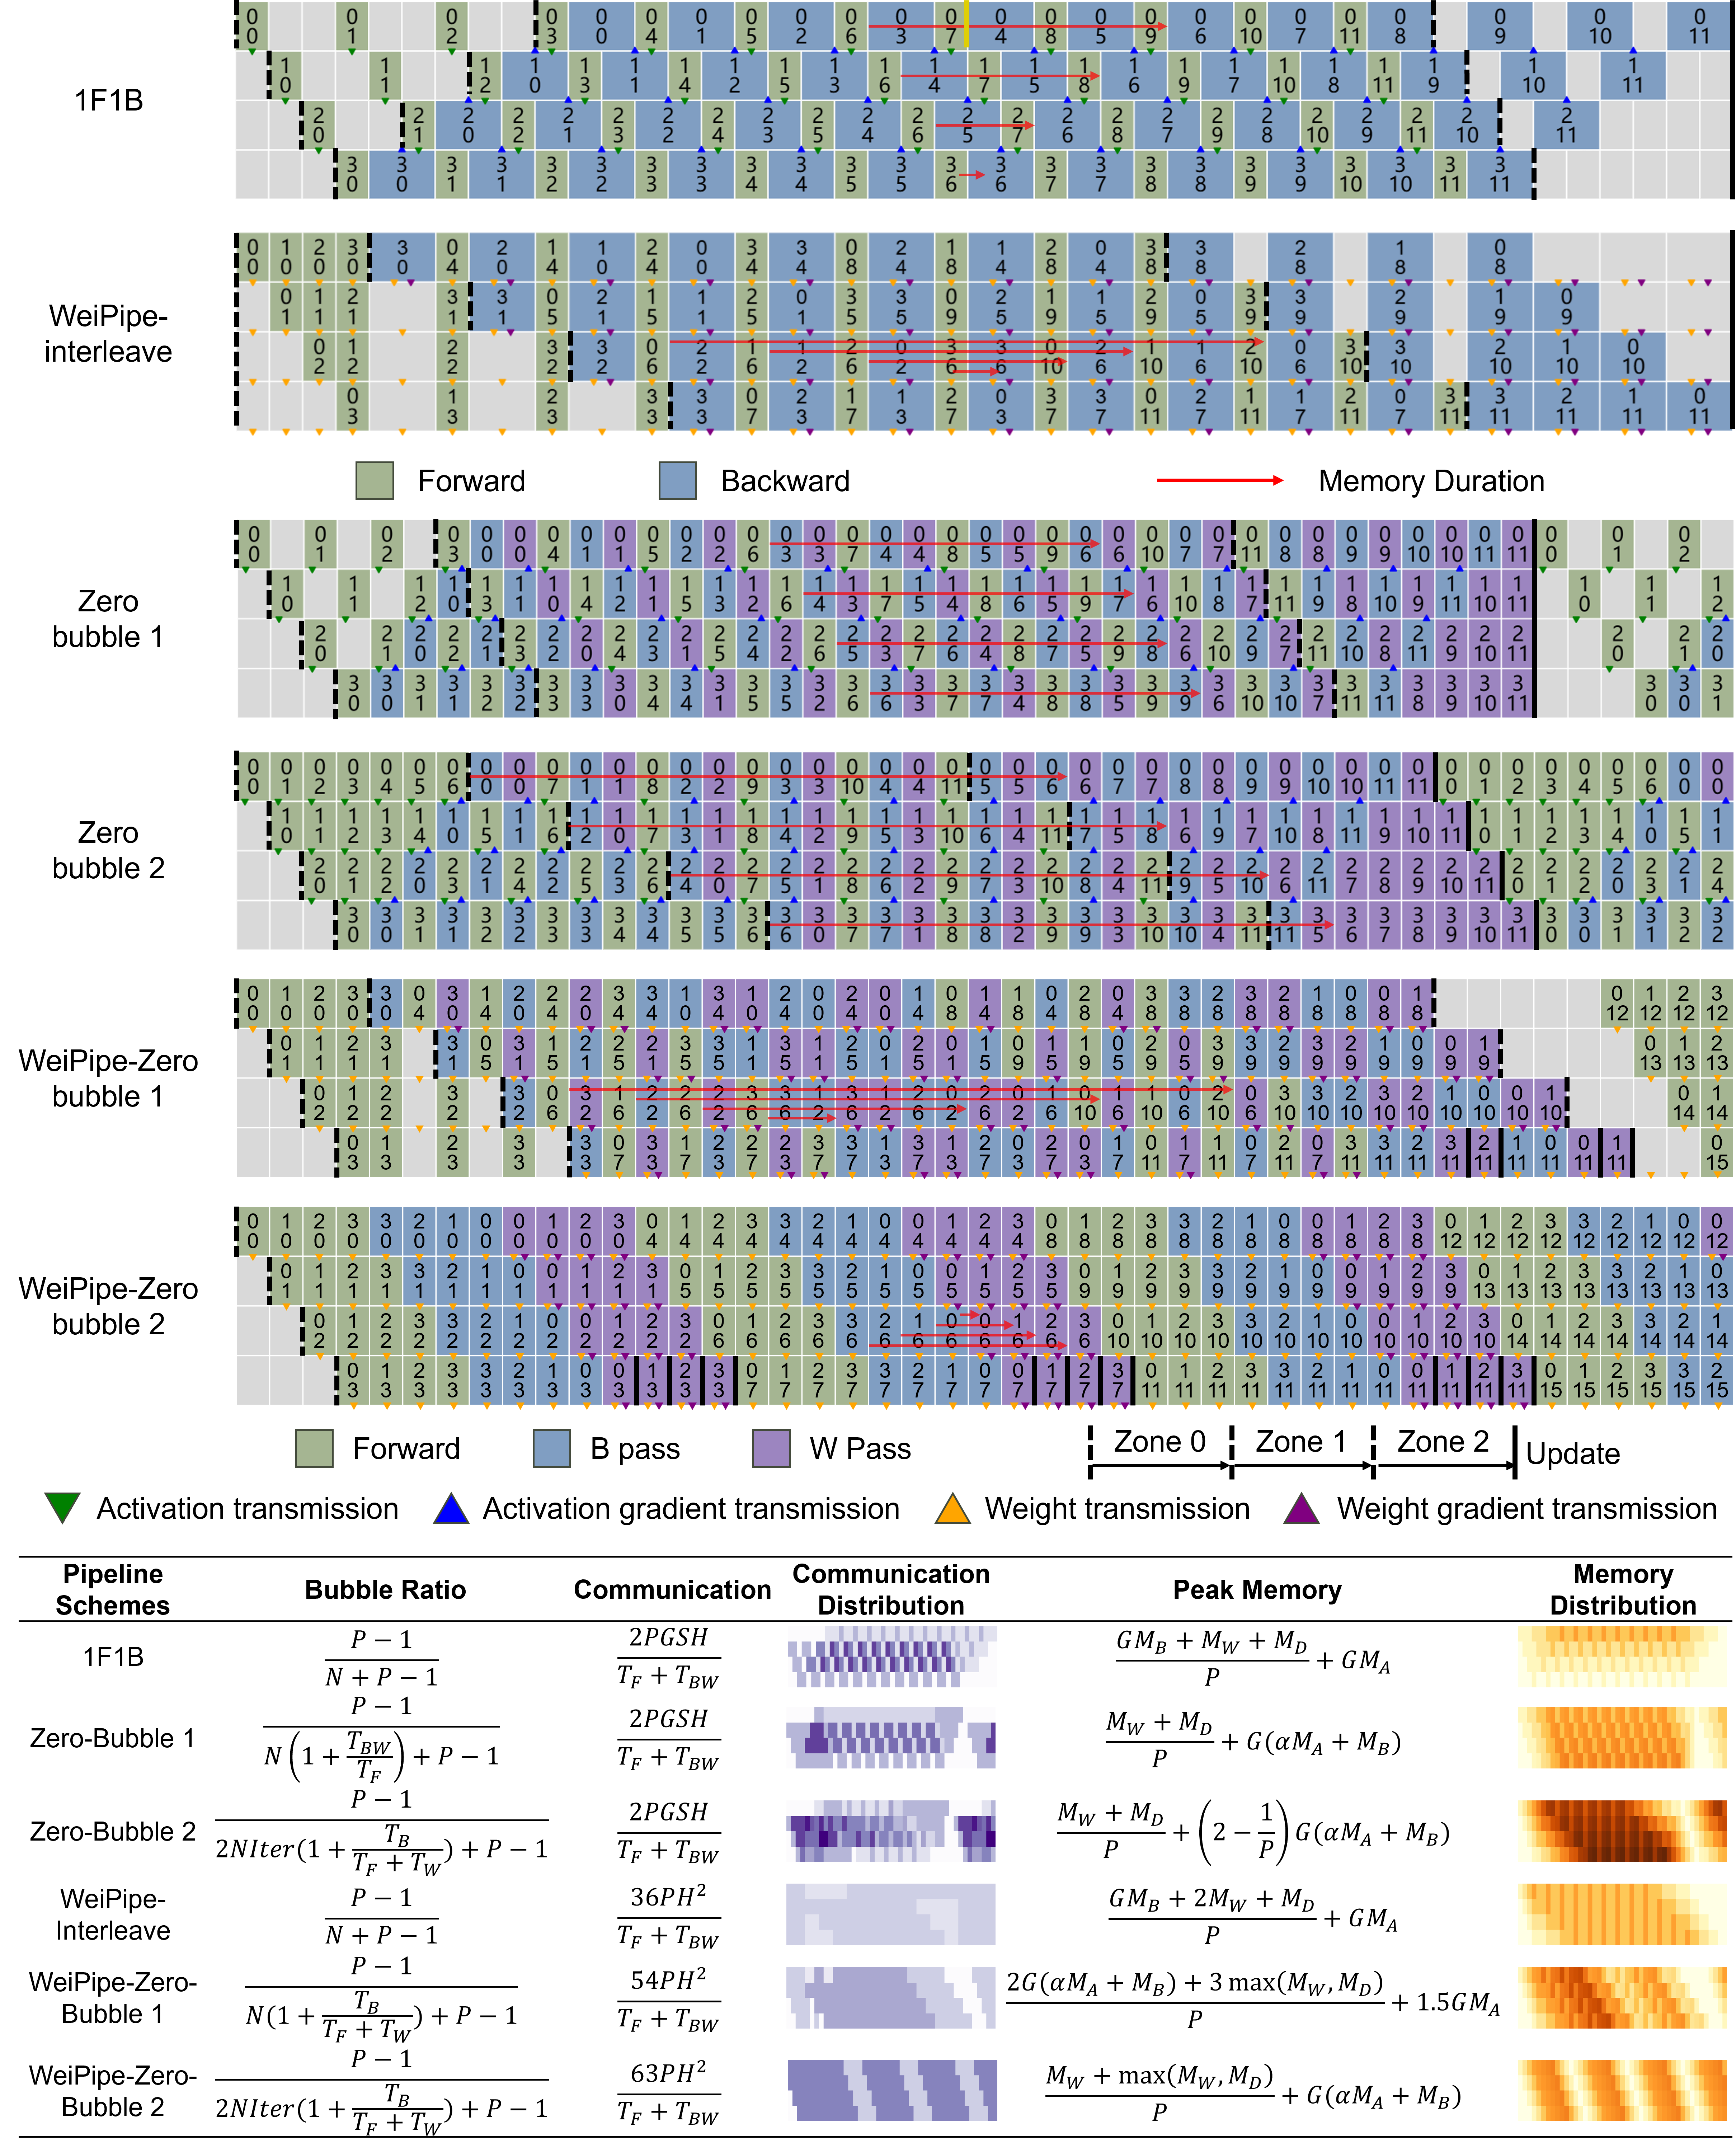
\includegraphics[width=\columnwidth]{figures/fig5.png}
    \caption{不同流水线策略在不同模型配置下的吞吐量对比。WeiPipe在长序列场景下展现出显著优势。}
    \label{fig:weipipe-throughput}
\end{figure}

图\ref{fig:weipipe-throughput}展示了不同策略的吞吐量对比。在NVLink环境下，WeiPipe在所有配置中均展现出比其他策略更高的性能。具体而言，当$H=4096$且$S=16384$时，WeiPipe相比1F1B和FSDP分别实现22.3\%和78.4\%的吞吐量提升。

在内存消耗方面，1F1B在所有流水线策略中内存使用最小。重计算和Flash Attention显著降低了1F1B和零气泡策略早期worker的内存使用。然而，如前述内存分析所解释的，零气泡方法在启用Flash Attention后的内存消耗显著高于1F1B——因为Flash Attention减少了注意力激活值，使前向激活值主要由FFN产生，B-pass产生的梯度大小接近前向激活值，导致最后一个worker的峰值内存约为1F1B的2倍。这在长上下文场景（$S \ge 8192$）中容易引发OOM错误，限制了零气泡策略的实用性。WeiPipe的内存使用略高于FSDP，主要来自通信缓冲区——WeiPipe-Interleave中每个worker需要分配三个接收缓冲区（用于接收$W$和$D$）和三个发送缓冲区，而FSDP以算子粒度创建更细粒度的缓冲区。

在PCIe和以太网互联环境下，WeiPipe-Interleave在$S=16384$且$H=2048, 4096$时，相比其他策略的最佳性能实现31.7\%和22.2\%的吞吐量提升。这一结果特别有价值，表明WeiPipe能够在资源受限环境中（如无法承担高端NVLink互联的团队和机构）显著降低对高带宽基础设施的依赖。需要指出的是，在NVLink环境下，WeiPipe的提升幅度相对小于PCIe环境，这是因为高带宽NVLink能够一定程度上掩盖传统PP的通信开销。

\begin{figure}[!t]
    \centering
    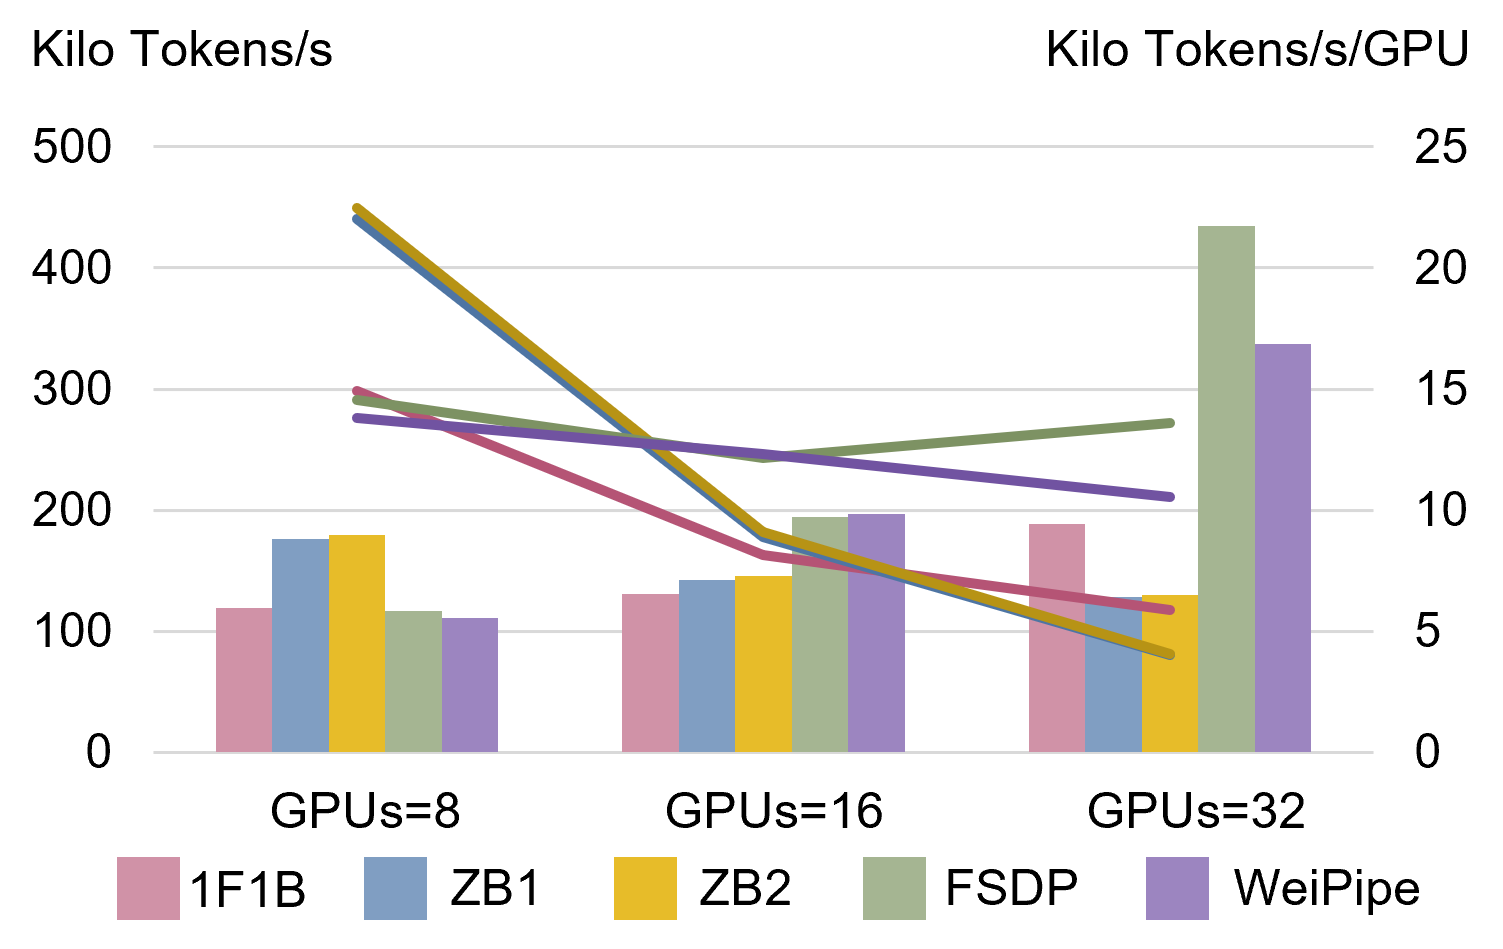
\includegraphics[width=\columnwidth]{figures/exp_fig3.png}
    \caption{不同序列长度下各策略的吞吐量对比。随着序列长度增加，WeiPipe的优势更加显著。}
    \label{fig:weipipe-seq-length}
\end{figure}

图\ref{fig:weipipe-seq-length}展示了不同序列长度下的性能对比。可以清楚地看到，随着序列长度从4K增加到128K，传统流水线策略的性能急剧下降，而WeiPipe的性能下降幅度远小于其他方法。这验证了WeiPipe将通信量与序列长度解耦的核心优势。

\subsection{可扩展性分析}

\begin{figure}[!t]
    \centering
    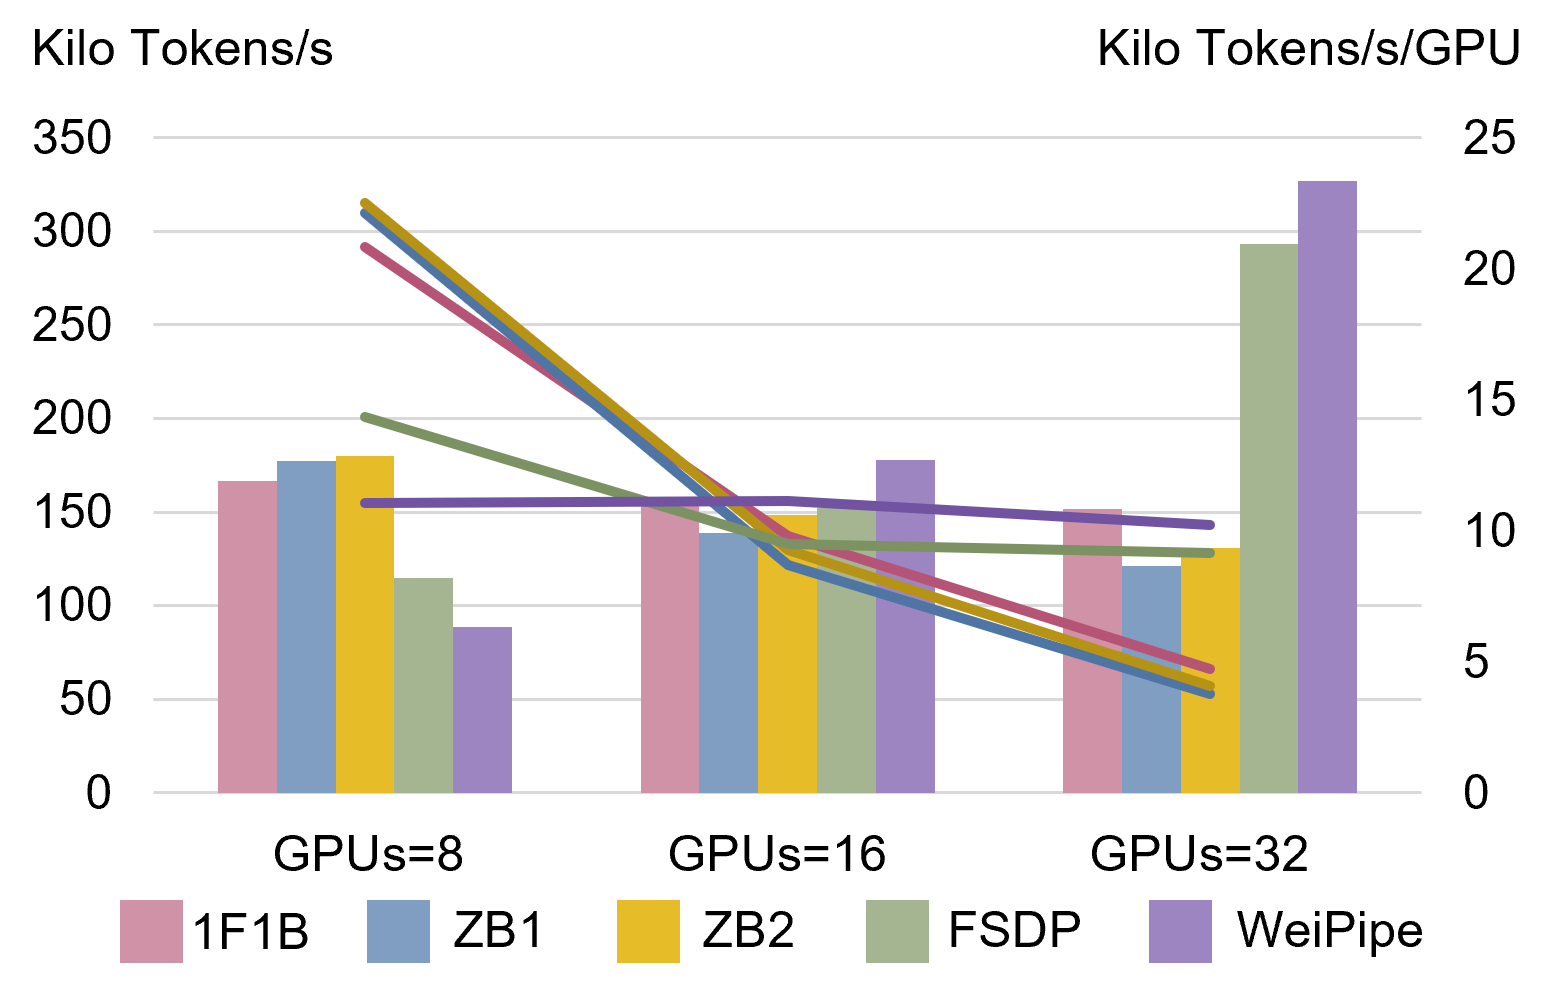
\includegraphics[width=\columnwidth]{figures/exp_fig4.png}
    \caption{WeiPipe的可扩展性分析。左图为弱扩展性，右图为强扩展性。WeiPipe在两种场景下都展现出良好的扩展特性。}
    \label{fig:weipipe-scalability}
\end{figure}

\textbf{弱扩展性}：通过保持每个worker的工作负载恒定，同时逐步增加worker数量（从8到32）和batch size（从128到512）来评估。固定序列长度为16384，层数为32，实验在32个A800 GPU（4个集群，集群内PCIe连接）上进行。图\ref{fig:weipipe-scalability}（左）的结果表明WeiPipe的整体性能与GPU数量的增加成比例扩展，验证了其弱扩展能力。与此形成对比的是，传统PP策略在更多GPU上性能提升受限，因为每个GPU处理的序列长度固定，激活值通信量不变，但随着更多GPU加入，通信频率增加，通信墙效应更加突出。

值得注意的是，在PCIe环境下WeiPipe-Interleave的弱扩展效率仍低于理想线性扩展。通过性能分析发现，主要瓶颈在于最后一次反向传播的尾部阶段：Worker 0在等待其他worker完成流水线的同时，还需要传输大块的权重数据，这种末尾的通信-计算串行无法完全隐藏，在扩展到更多GPU时影响会逐步显现。未来可通过进一步优化末尾阶段的通信调度来改善。

\textbf{强扩展性}：保持任务规模恒定（batch size固定为128），同时扩展worker数量从8到32，测试相同总工作量下多GPU的加速比。图\ref{fig:weipipe-scalability}（右）的结果表明WeiPipe相比其他策略展现出优越的可扩展性。长序列长度和低带宽通信基础设施（PCIe+以太网）给传统PP方法带来严重的通信压力：当GPU数量从8增加到32时，传统PP方法的通信墙效应线性放大，而WeiPipe的通信量与序列长度无关，仅随GPU数增加通信次数而非通信量。这使得WeiPipe在强扩展场景下展现出利用更多GPU实现更大加速的潜力，其扩展效率（实际加速比/理想线性加速比）显著高于1F1B和FSDP，尤其是在更高GPU数量和更长序列长度的组合下。

\section{本章小结}

本章针对长上下文大模型训练中的通信瓶颈问题，提出了权重流水线并行新范式WeiPipe。通过突破传统流水线并行"传递激活值"的范式，WeiPipe将通信量从与序列长度相关解耦为仅与模型大小相关，从根本上解决了长序列场景下的通信挑战。

本章的主要贡献包括：（1）提出权重流水线并行的理论基础，分析了传递权重比传递激活值更高效的临界条件；（2）设计了WeiPipe-Naive、WeiPipe-Interleave和WeiPipe-zero-bubble三种策略，实现了从基础到高级的完整方案；（3）通过实验验证了WeiPipe在长序列场景下相比传统方法的显著性能优势，在通信受限环境中展现出更好的可扩展性。

WeiPipe扩展了使用流水线并行训练长上下文模型的前景，并降低了对昂贵高带宽通信基础设施的依赖。这对于资源受限环境下的大模型训练具有重要意义。随着大模型向更长上下文方向发展（如1M tokens甚至更长），WeiPipe所提供的通信效率优势将变得更加关键。未来，WeiPipe的权重流转思想可以与其他并行策略（如张量并行、序列并行）进一步结合，为超大规模长上下文模型的训练提供更全面的解决方案。
